\documentclass[letterpaper]{article}
% Author order, affiliations, and emails supplied by the authors.
% Confirm the corresponding author and review mode before submission.
\usepackage[draft]{aaai2027}
\usepackage[hyphens]{url}
\usepackage{graphicx}
\urlstyle{rm}
\def\UrlFont{\rm}
\usepackage{natbib}
\usepackage{caption}
\usepackage{booktabs}
\frenchspacing
\pdfinfo{/TemplateVersion (2027.1)}
\setcounter{secnumdepth}{0}

\title{CyberGraph: Interactive Security Review with\protect\\ Code Knowledge Graphs and Evidence-Grounded Answers}
\author{
Azizur Rahman\textsuperscript{1}, Laraib Hasan\textsuperscript{1}, Rushikesh Hiray\textsuperscript{1}, Shubham Srivastava\textsuperscript{1},\\
Mohammad Hijjawi\textsuperscript{1}, Jafar Rahman\textsuperscript{2}, Harshit Taneja\textsuperscript{1}
}
\affiliations{
\textsuperscript{1}University of Birmingham \quad \textsuperscript{2}Independent Researcher\\
er.azizurrahman@gmail.com, laraib.hasan45@gmail.com, rhiray03@gmail.com\\
shubham03workplace@gmail.com, mohammad.hijjawi1997@gmail.com\\
rahmanjafar2004@gmail.com, hxt532@student.bham.ac.uk
}

\begin{document}
\maketitle

\begin{abstract}
CyberGraph connects exposed routes, controls, and sensitive operations through
a local security knowledge graph, an offline explorer, and evidence-grounded
question answering. Language-specific analyzers populate a shared graph;
bounded call traversal identifies potential entrypoint-to-sink paths. Retrieved
records expose citations and heuristic confidence. Answers are deterministic
by default, with optional language-model phrasing. We demonstrate a review loop
on the public PyGoat training application: build the graph, inspect a
SQL-injection path, ask a cited question, parameterize the query, and compare
scans. The repair removes one finding while the system retains a REVIEW
verdict. The demonstration emphasizes auditable evidence and explicit
uncertainty rather than automatic claims of program safety.
\end{abstract}

\begin{links}
    \link{Code}{https://github.com/AQ-Labs/cybergraph}
\end{links}

\begin{figure*}[t]
\centering
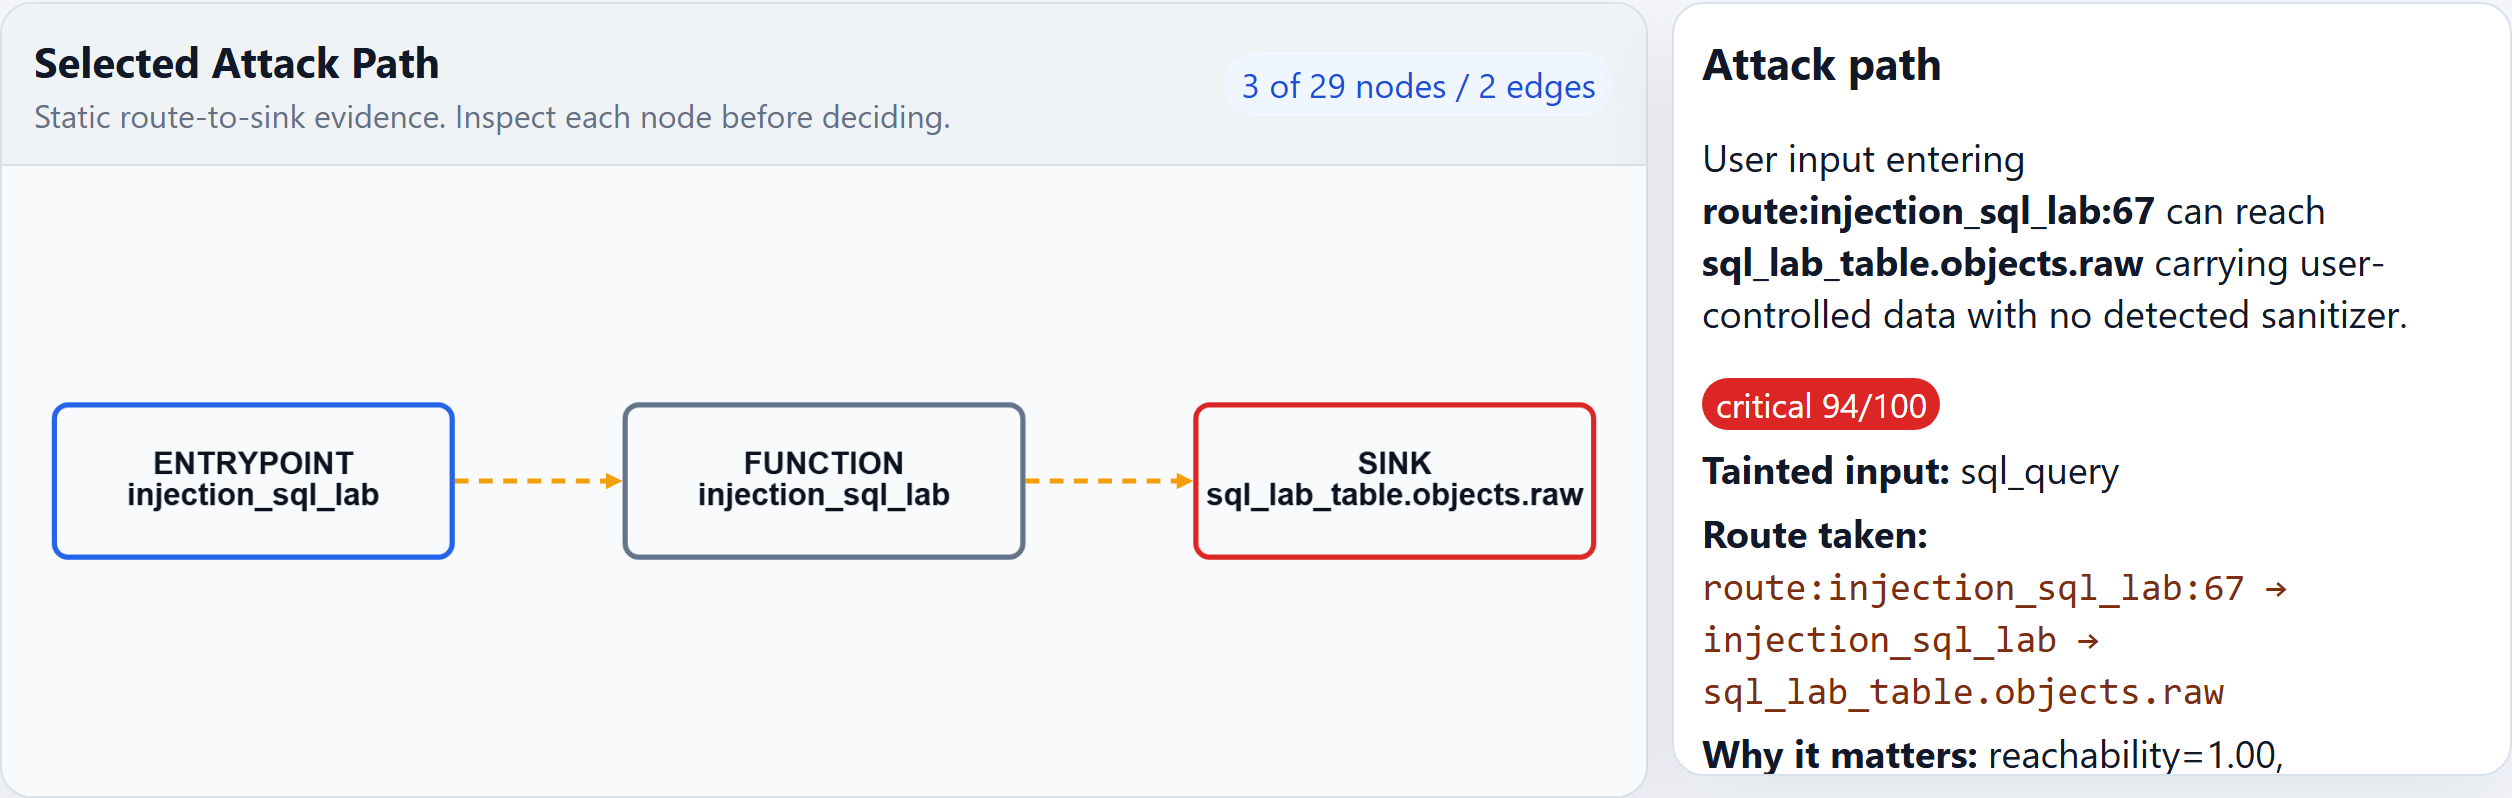
\includegraphics[width=\textwidth]{figures/explorer.png}
\caption{Actual offline explorer on PyGoat, with typography scaled for print.
Selecting a path isolates the entrypoint, handler, and SQL sink; the scrollable
evidence panel exposes its rationale. The displayed 94/100 is a review-priority
heuristic, not an exploitation probability. Source drill-down supports verification.}
\label{fig:workflow}
\end{figure*}

\section{Motivation and Related Work}
Reviewers need to connect a suspicious call to its entrypoint, controls, and
source, then check what changes after a repair. CyberGraph integrates this
workflow with graph-backed explanations, not a claim of stronger detection.

Code property graphs support vulnerability-oriented traversal
\citep{yamaguchi2014}; CodeQL provides data-flow analysis \citep{codeql}, and
FlowDroid models Android lifecycle-aware taint propagation \citep{arzt2014}.
CyberGraph's lightweight graph does not claim their analysis precision.
Devign learns graph-based vulnerability classifiers \citep{zhou2019}, while
LineVul predicts vulnerable lines using transformers \citep{fu2022}.
CyberGraph instead exposes extracted evidence for interactive review.

Retrieval-augmented generation conditions answers on retrieved information
\citep{lewis2020}. GraphRAG uses LLM-derived entity graphs and community
summaries for corpus-level questions \citep{edge2025}; CyberGraph retrieves
typed code records and paths, without requiring LLM-based graph construction.
Unlike work on LLM-generated vulnerability repairs \citep{pearce2023}, this
demo applies a predefined patch and inspects its effects. These are
methodological distinctions, not head-to-head performance comparisons.

The contribution is an inspect--question--repair--recheck interaction: a
developer explores a path, queries the same graph-derived evidence, and checks
the effect of a patch. The AI-facing component is structured retrieval for
optional neural explanation; neither extraction nor the demonstrated answers
require a model. We assess what path records add through a small retrieval
ablation, not a claim of a new detection algorithm or measured developer gains.

\section{System Architecture}
\textbf{Extraction and storage.}
The Python CLI dispatches analyzers for Python, JavaScript/TypeScript, Go,
Java, and C\#. Python uses its abstract syntax tree; other adapters use
lightweight structural and pattern-based extraction. Framework coverage varies.
A shared contract stores nodes, edges, and findings in SQLite. Relationships include
\texttt{EXPOSES\_ENTRYPOINT}, \texttt{GUARDS}, \texttt{SANITIZES},
\texttt{CALLS\_RESOLVED}, and \texttt{REACHES\_SINK}. File/line metadata links
evidence to source. Optional scanner imports add findings and advisories.

\textbf{Path analysis and uncertainty.}
Call resolution links candidate definitions across files. Bounded breadth-first
traversal follows these links from entrypoints to sinks. Paths retain the
weakest call-resolution confidence, sanitizer markers, and available local
taint evidence. These signals prioritize inspection, not prove exploitation;
a function-level control need not protect every execution. Change checks
distinguish failures, unknown results, and unsupported capabilities. Their
\textsc{Accept}/\textsc{Review} decision is separate from the CI gate:
\textsc{Accept} concerns checks run, not whole-program safety.

\textbf{Grounded answers and presentation.}
The \texttt{explain} command classifies questions by keywords and ranks records
by category agreement and lexical overlap, favoring findings and paths.
Records carry file/line or path citations. Local answers mark empty retrieval
as insufficient evidence and related-only evidence as inconclusive. Confidence
is heuristic, not calibrated. Optional Anthropic, OpenAI, or Kimi clients
receive numbered evidence and citation instructions, not a guarantee against
unsupported generation. Default answers are assembled locally.
The offline HTML explorer uses Cytoscape.js \citep{franz2016} for security-layer
views, search and severity filters, focused paths, and source drill-down.
JSON, SARIF, and optional MCP integration expose the evidence to other tools.
Suppressed findings can retain underlying graph evidence for inspection.

\section{Interactive Demonstration}
The under-five-minute walkthrough uses PyGoat, an intentionally vulnerable
Django training application \citep{pygoat}, at commit \texttt{19d17cc}.
The vulnerable application is neither started nor exploited.
Figure~\ref{fig:workflow} shows the running interface.

\textbf{1. Build the graph.}
After installation and cloning the target, the presenter runs
\texttt{cybergraph doctor .} and \texttt{cybergraph quickstart .}.
The latter creates configuration and a GitHub Actions workflow,
with the database and \texttt{report.html} in \texttt{.cybergraph/}.
Explicit exports produce \texttt{graph.json} and \texttt{findings.sarif}.
Source snippets are opt-in because reports may disclose repository content.

\textbf{2. Inspect a path.}
The baseline contains 806 stored nodes, 2,634 edges, and 14 findings.
The presenter selects the SQL path from a Django route
in \texttt{urls.py:67}, through \texttt{injection\_sql\_lab}, to
\texttt{sql\_lab\_table.}\allowbreak\texttt{objects.raw} in \texttt{views.py:878}.
The focused view isolates role-labeled nodes and directional edges. Source
evidence shows request parameters at lines
858--859 and string-built SQL at line 864. Authentication at line 856 does not
make this SQL construction safe. Attendees can inspect other paths and source.

\textbf{3. Ask and repair.}
The presenter asks \texttt{explain} to trace the handler to the sink.
The local response cites the path and sink line and recommends parameterization.
The presenter replaces string concatenation with placeholders and a parameter
list, then runs
\texttt{cybergraph analyze .} and \texttt{cybergraph history .}.
Findings decrease from 14 to 13, with no new or regressed findings.
The verdict remains \mbox{\textsc{Review}}: unsafe calls and configuration
warnings remain. A static path can persist after parameterization because
structural reachability and a vulnerability verdict are different outputs.

\textbf{Delivery.}
Attendees choose paths and questions on a laptop, inspect citations, and
observe scan changes. Pinned code, prebuilt reports, and video provide an
offline fallback. Model calls and CI uploads are optional and not demonstrated.

\section{Evidence, Scope, and Limitations}
\textbf{Regression check.} At revision \texttt{b3b47b1} (analysis base
\texttt{18329a6}), the existing 11 seeded reachability cases yield 9 true
positives, 0 false positives, and 0 false negatives by expected endpoint/sink
label matching. Nine positives span Python, Go, and Java; two negatives cover
Python and Go. This checks consistency, not every intermediate edge or
real-world detection accuracy. Dataset artifacts can distort vulnerability
evaluation \citep{chakraborty2022}.

\textbf{Retrieval ablation.} For each of the nine positive cases, we ask
``What sensitive sink is reachable from [entrypoint]?'' using its existing
expected label. Ranking is unchanged across three record pools, with at most
two complete records and 2,000 characters per question. Both expected endpoint
labels occur in retrieved evidence for 0/9 questions with findings only, 8/9
without path records, and 9/9 with path records. Only the last condition
returns connected path citations (9/9). Mean context lengths are 136, 243,
and 544 characters, respectively. These are seeded, template-generated
questions: label co-occurrence is not relationship correctness, and the
larger context is a confound. The saved protocol, per-question records, and
runner make this descriptive evidence-availability comparison reproducible;
it is neither a held-out benchmark nor an LLM evaluation.

The PyGoat loop is not a user study or new vulnerability discovery. The repair
was syntax-checked, not database-tested. Dynamic dispatch, missing framework
models, function-level control markers, and bounded traversal can produce
missed or misleading paths. External LLMs receive selected context only when
enabled; citation instructions do not guarantee faithful generation. Broader
labeled-repository evaluation, model faithfulness tests, and usability studies
remain future work.

\bibliography{references}
\end{document}
